\section{Ergebnisse und Berechnungen}
\label{sec:ergebnisse}
%Tabelle START

%Tabelle START
\vspace*{-2.5mm}
\renewcommand{\arraystretch}{1.2}
\begin{table}[h!]
	\centering
	\caption{Messergebnisse der untersuchten Proben}
	\label{tab:Messergebnisse der untersuchten Proben}
	\resizebox{15cm}{!}{
	\begin{tabulary}{1.1\textwidth}{C|C|C|L}
%		\hline
%		\multicolumn{3}{|c|}{Automatisch }\\
		\hline
		\textbf{Stoff}& \textbf{Flammpunkt}& \textbf{Gefahrenklasse} & \textbf{Begründung}\\
		\hline
		Wein & \SI{45}{\celsius} & R10/H226 & Flammpunkt zwischen 21 bis \SI{25}{\celsius} - entzündliche Flüssigkeit\\
		Unbekanntes Ethanol & \SI{45}{\celsius} & R10/H226 & Flammpunkt zwischen 21 bis \SI{25}{\celsius} - entzündliche Flüssigkeit\\
		Diesel & \SI{61}{\celsius} & - & Flüssigkeit mit Flammpunkt über \SI{55}{\celsius}\\
		Wasser-Ethanol- Gemisch (\SI{12}{\volp}) & \SI{47}{\celsius} & R10/H226 & Flammpunkt zwischen 21 bis \SI{25}{\celsius} - entzündliche Flüssigkeit\\
		\hline
	\end{tabulary}
	}
\end{table}
\FloatBarrier 
\vspace*{-4mm}
%Tabelle ENDE
%Start
\begin{figure}[h!]
	\centering
	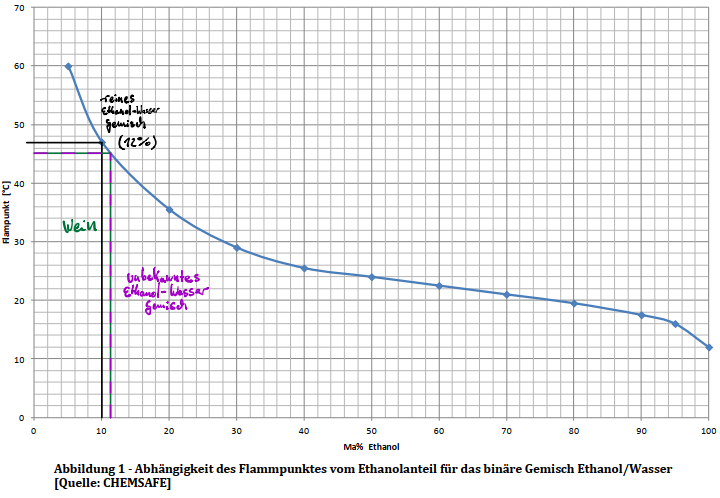
\includegraphics[width=0.75\textwidth]{img/Diagramm}
	\caption{Flammpunkt in Abhängigkeit vom Ethanolanteil}
	\label{fig:dia}
\end{figure}
\FloatBarrier
%Ende

\subsection*{Bestimmung von Gewichts- und Volumenanteil der unbekannten Ethanolprobe}

Der in der Abbildung \ref{fig:dia} eingetragene Flammpunkt von \SI{42}{\celsius} lässt, mit der blau eingetragenen Abhängigkeit, einen Massenanteil der unbekannten Ethanol-Probe von \SI{12}{\volp} bestimmen.
\begin{flalign}
m_{\ce{Et}} 	&= m*\chi_{\ce{Et}}\\
&= \SI{1}{\kg}*\SI{12}{\percent}\\
&=\underline{\SI{0,12}{\kg}}
\end{flalign}
\begin{flalign}
m_{\ce{H2O}} 	&= m*\chi_{\ce{H2O}}\\
&= \SI{1}{\kg}*\SI{88}{\percent}\\
&= \underline{\SI{0,88}{\kg}}
\end{flalign}
\begin{flalign}
V_{\ce{Et}}		&= \frac{m_{\ce{Et}}}{\rho_{\ce{Et}}}\\
&= \frac{\SI{0,10}{\kg}}{\SI{0,789}{\kg\per\liter}}\\
&= \underline{\SI{0,152}{\liter}}
\end{flalign}
\begin{flalign}
V_{\ce{H2O}}	&= \frac{m_{\ce{H2O}}}{\rho_{\ce{H2O}}}\\
&= \frac{\SI{0,88}{\kg}}{\SI{1,000}{\kg\per\liter}}\\
&= \underline{\SI{0,880}{\liter}}
\end{flalign}
\begin{flalign}
V\%_{\ce{Et}}	&= \frac{V_{\ce{Et}}}{V_{\ce{Et}}+V_{\ce{H2O}}}\\
&= \frac{\SI{0,152}{\liter}}{\SI{0,152}{\liter}+\SI{0,880}{\liter}}\\
&\approx \underline{\SI{15}{\percent}}
\end{flalign} 

Die Umrechnung in Volumenprozent zeigt, dass sich für die gemessene unbekannte 
Ethanol-Probe ein Volumengehalt von \SI{15}{\volp} bestimmen lässt.
\subsection*{Vergleich der Weinprobe mit der Rein-Ethanol-Wasser-Mischung}
In Abbildung 1 ebenfalls eingetragen sind die Flammpunkte von je \SI{45}{\celsius} für das alkoholischen Getränk (Wein, Angabe \SI{12}{\volp}) und dem Rein-Ethanol-Wasser-Gemisch (angemischt \SI{12}{\volp}) mit einem Flammpunkt von \SI{47}{\celsius}. 
Aus Abbildung 1 ergeben sich daraus für das alkoholische Getränk \SI{12}{\mpp} Ethanol und für das Rein-Ethanol-Wasser-Gemisch \SI{10}{\volp}Ethanol.\\
\newpage
\textbf{Rückrechnung des Ethanol-Wasser-Gemisches von Massen- auf\linebreak Volumenprozent}
\begin{flalign}
m_{\ce{Et}} 	&= m*\chi_{\ce{Et}}\\
&= \SI{1}{\kg}*\SI{10}{\percent}\\
&=\underline{\SI{0,10}{\kg}}
\end{flalign}
\begin{flalign}
m_{\ce{H2O}} 	&= m*\chi_{\ce{H2O}}\\
&= \SI{1}{\kg}*\SI{90}{\percent}\\
&= \underline{\SI{0,90}{\kg}}
\end{flalign}
\begin{flalign}
V_{\ce{Et}}		&= \frac{m_{\ce{Et}}}{\rho_{\ce{Et}}}\\
&= \frac{\SI{0,10}{\kg}}{\SI{0,789}{\kg\per\liter}}\\
&= \underline{\SI{0,127}{\liter}}
\end{flalign}
\begin{flalign}
V_{\ce{H2O}}	&= \frac{m_{\ce{H2O}}}{\rho_{\ce{H2O}}}\\
&= \frac{\SI{0,90}{\kg}}{\SI{1,000}{\kg\per\liter}}\\
&= \underline{\SI{0,900}{\liter}}
\end{flalign}
\begin{flalign}
V\%_{\ce{Et}}	&= \frac{V_{\ce{Et}}}{V_{\ce{Et}}+V_{\ce{H2O}}}\\
&= \frac{\SI{0,127}{\liter}}{\SI{0,127}{\liter}+\SI{0,900}{\liter}}\\
&\approx \underline{\SI{12}{\percent}}
\end{flalign} 
Laut der Angabe auf der Weinverpackung mit \SI{12}{\volp} erwarten sich für das angesetzte 
Rein-Ethanol-Wasser-Gemisch und der alkoholischen Getränkeprobe dieselben Messwerte. Dies ist nicht der Fall. Das angesetzte Ethanol-Gemisch entspricht mit \SI{1}{\mpp} und den daraus berechneten \SI{12}{\volp} der Erwartung für die Flammprobe. Die Weinprobe ist jedoch mit \SI{12}{\mpp} und den sich daraus ergebenden \SI{15}{\volp} über dem Erwartungswert von \SI{12}{\volp}.\\
Grund für diese Abweichungen der alkoholischen Weinprobe könnten Fuselalkohole 
(z.B. Methanol, Propanol) sein, welche nicht dem Ethanol entsprechen, jedoch die Flammbarkeit des Weines selbst beeinflussen. So könnten diese Alkohole den Flammpunkt herabsetzen und damit eine verfälschte Bestimmung mit einem höheren Volumenanteil an Ethanol bewirken.
